\section{Client-Server Architecture}

One of the first technical design decisions that was discussed was that of the client-server architecture and how the different clients would keep synchronised with each other. This was a very important decision to make as a poor networking set up can severely impact the playability of the game. For example, Patrick Wyatt talks about how the first ever multiplayer game of \emph{Warcraft} experienced a serious game-state synchronisation problem; both computers involved ended up ``showing entirely different battles that, while they started identically, diverged into two entirely different universes''.\cite{wyatt2012warcraft} Three separate strategies for solving this problem were discussed: lockstep, simple server-client, and server-client with simulation.

Lockstep is a peer-to-peer strategy in which each computer has a full model of the game state. Whenever the world changes on one of the clients involved with the game, they must update their own game state and then send this update to all of the other clients to apply to their copies of the game state too. There is no centralised server in this networking model, so disconnection of a single client does not cause the game to stop. It also allows users to play games on networks with high latency without actually experiencing any perceived lag. This is because when packets are delayed the client is able to continue to play the game and apply the update whenever it arrives. The robustness afforded by this technique is highly desirable for games with long playing times, such as Sid Meier's Civilisation.\sidenote{Sid Meier's Civilization is a turn-based strategy game, for more information see \url{civilization.com}.}

However, maintaining synchronisation when using a peer-to-peer protocol like this can be very challenging. The clients have to be able to collectively handle messages arriving in different orders for each individual. If this happens the game can start to desynchronise and the games will ultimately diverge. For example, Figure~\ref{fig:serverClientDesync} shows how two clients can easily diverge. Each row in the diagram shows the state of the game for each client, with client one on the left and client two on the right, at the given time step. Client one sees the blue character successfully hit the red character, but client two sees the red character step out of the way and the blue player's shot misses.

\begin{marginfigure}
	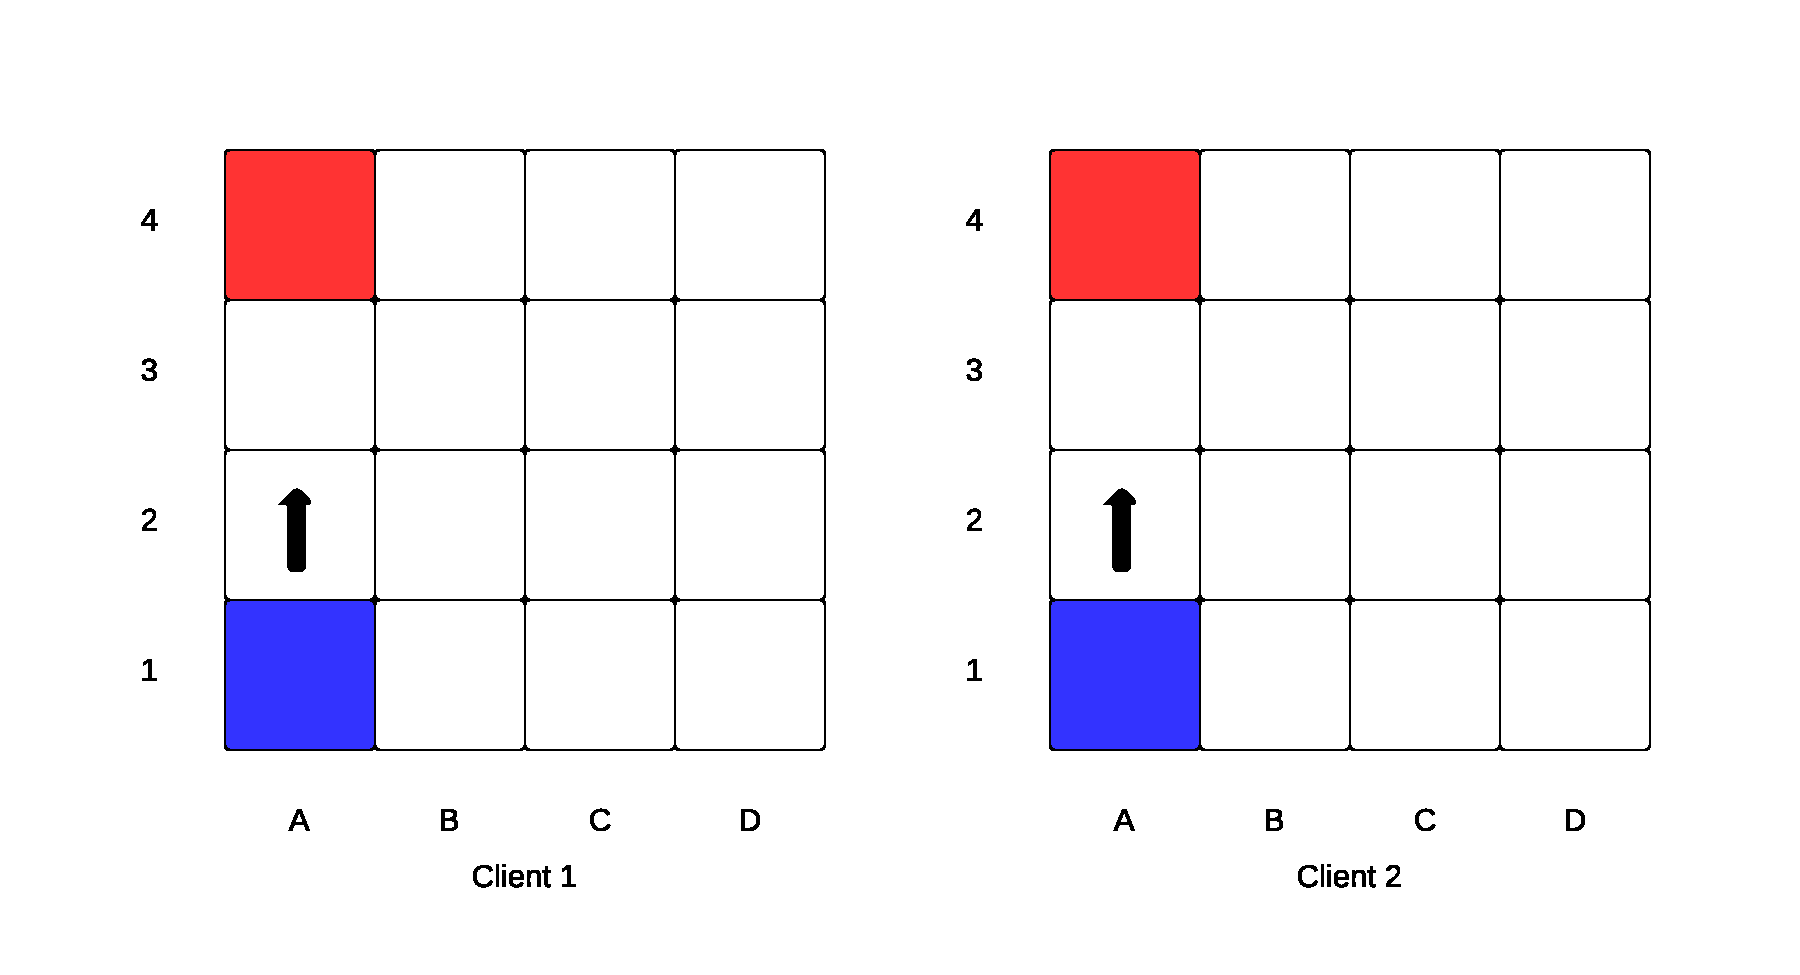
\includegraphics{res/computer_communication_architecture/ServerClientDesynchronisation1.pdf}
	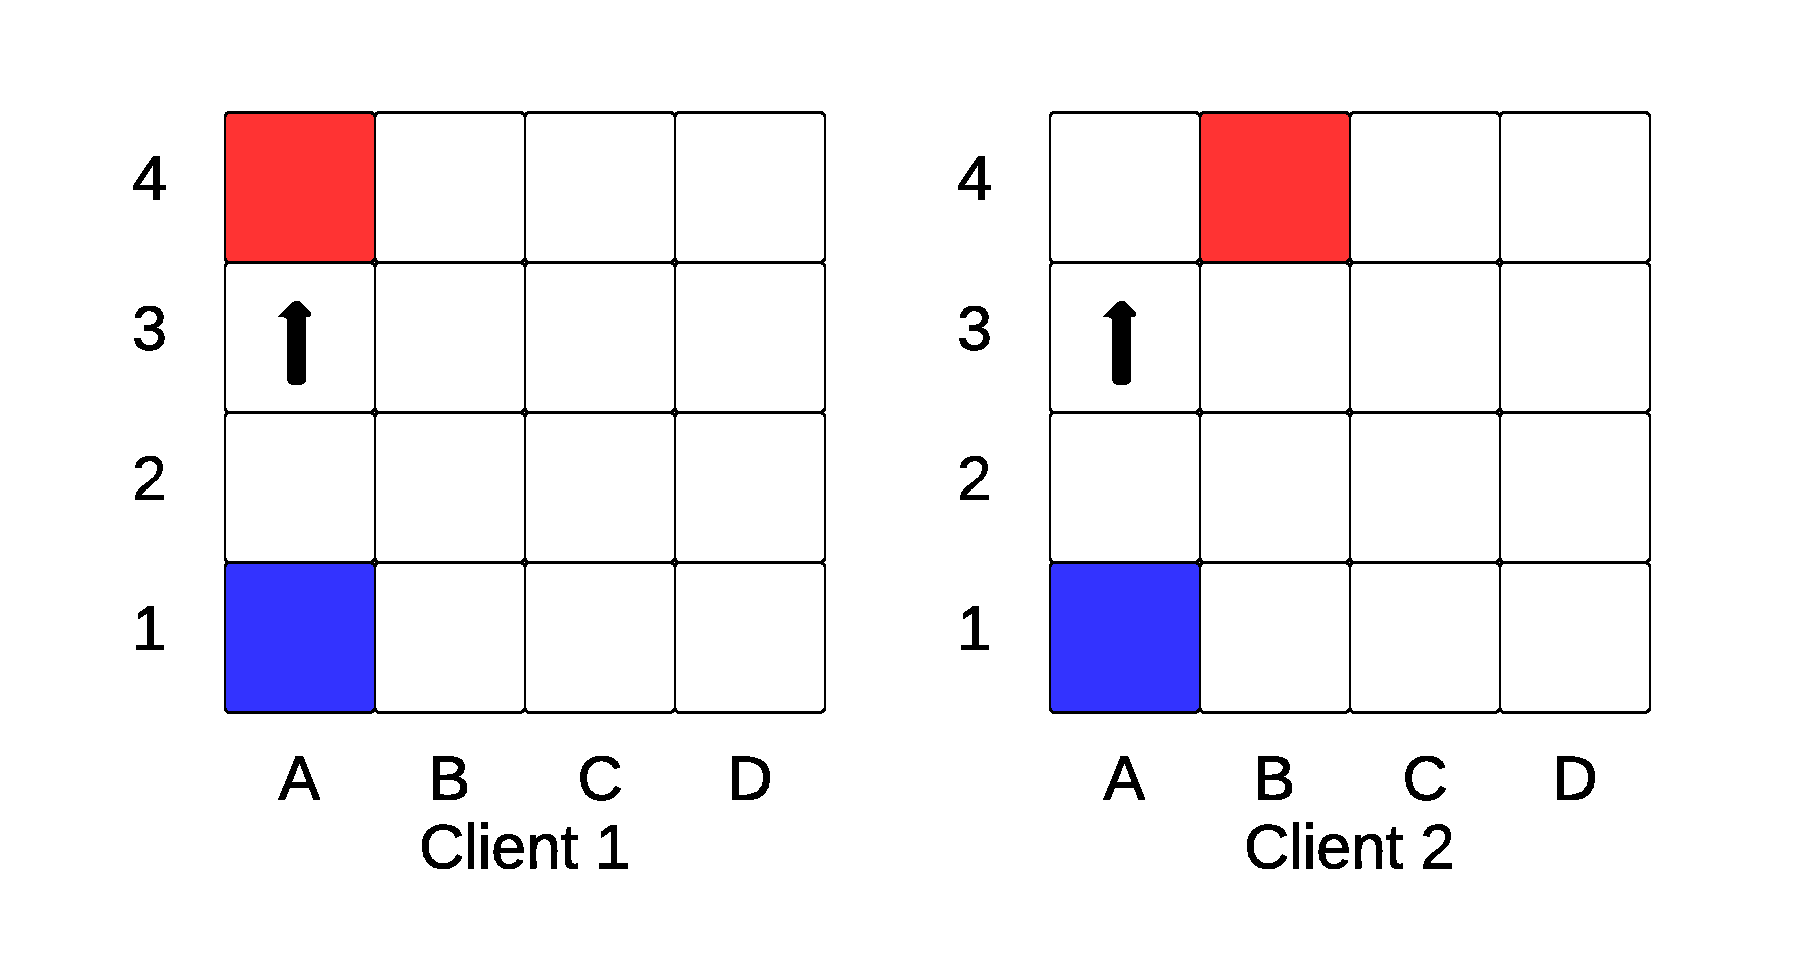
\includegraphics{res/computer_communication_architecture/ServerClientDesynchronisation2.pdf}
	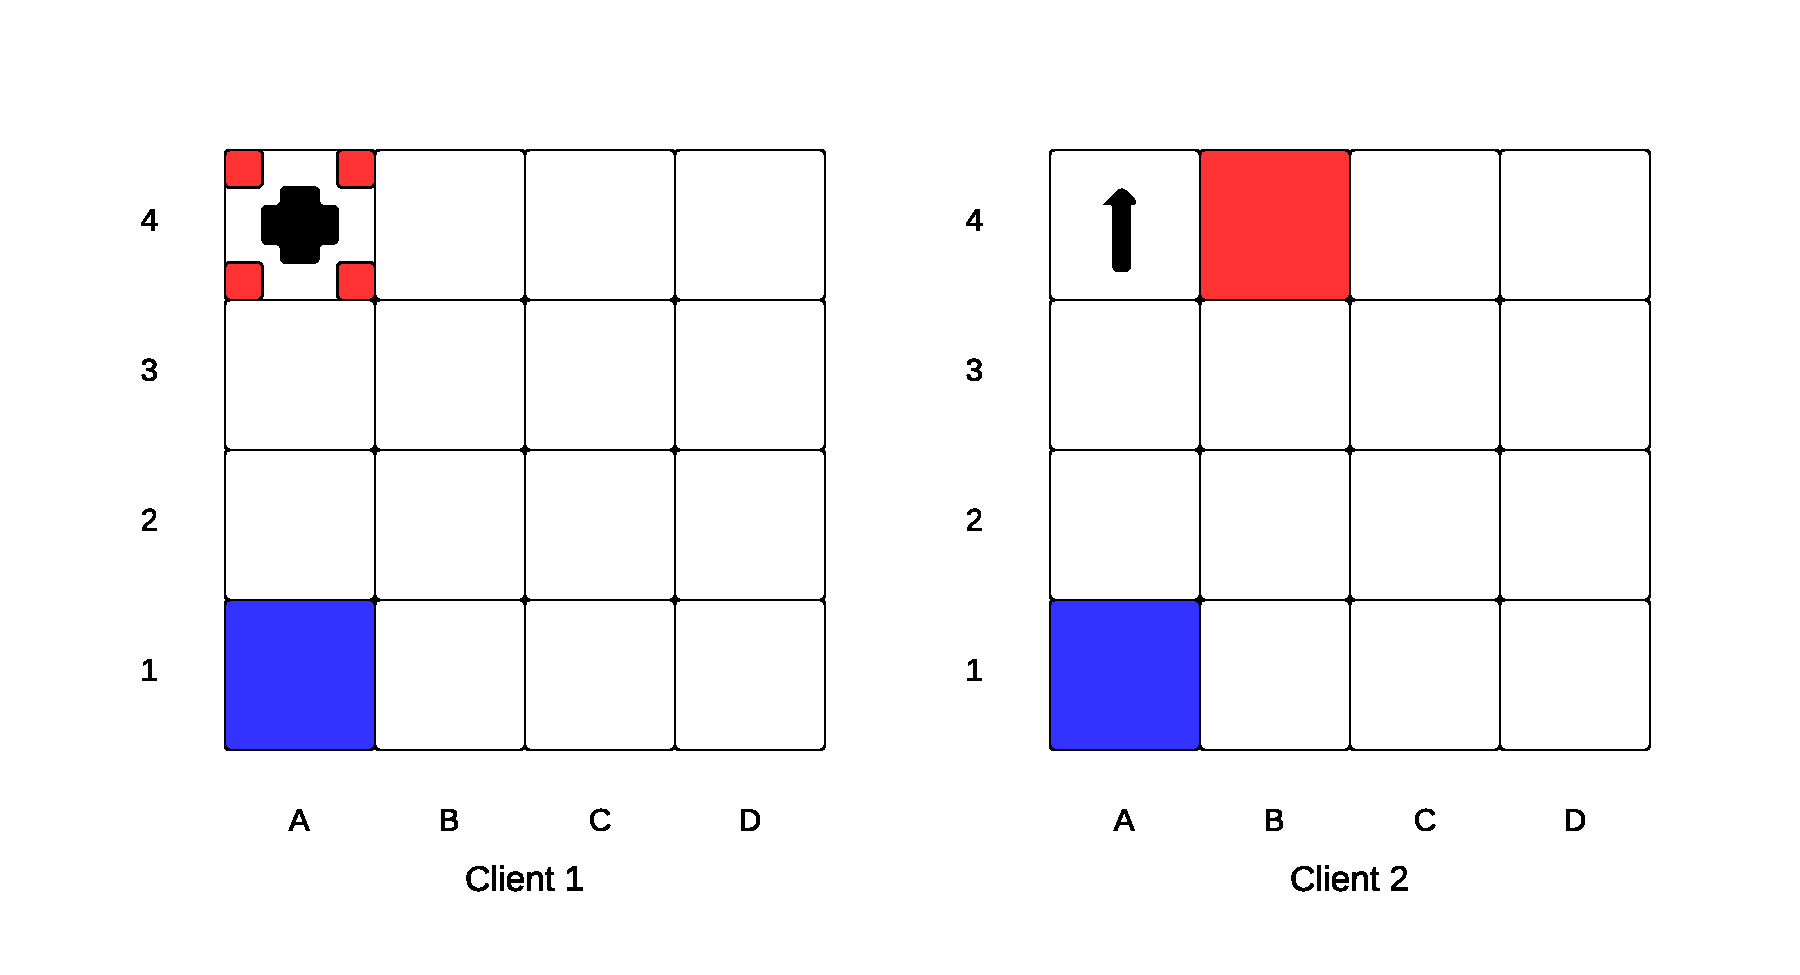
\includegraphics{res/computer_communication_architecture/ServerClientDesynchronisation3.pdf}		
	\caption[Desynchronisation when using lockstep]{Example of desynchronisation when using a lockstep strategy.} Client 1 on left, client 2 on right. 
	Each diagram represents state of game for that clients at a given time period.	3 diagrams vertically aligned, First one is top, second one is middle, third one is bottom.
	\label{fig:serverClientDesync}
\end{marginfigure}

In the simple server-client model the server and each of the clients have a copy of the game state, but instead of sharing the updates in a peer-to-peer fashion the server holds the master copy and it distributes canonical updates to the clients. When a player performs an action, the client sends a message to the server informing it of what happened. The server then applies the action to the game state to create an update which it sends to all of the clients. It must be ensured that all update messages are applied in the correct order, but this is much simpler to solve compared to the peer-to-peer version of the same problem since one machine is in charge of the decisions instead of a collective of machines.

The drawback to this approach is that clients must wait for the server to provide updates before they can show the new game state to the users. This can cause considerable lag when the network has high latency or is experiencing loss.

The final strategy was server-client with simulation. This is similar to simple server-client in that each node has a copy of the game state, but the server's is deemed to be the master copy. However, clients also perform some simulation using client side prediction of the events about to occur in the very near future. If the client side prediction is incorrect then the authoratitive version of the game state held by the server will eventually correct the client's local state. This helps compensate for any latency on the network. The downside is that there can be noticeable changes in the game state if a correction is not received until a long time after the initial client side prediction failure occured. This strategy is popular with modern first person shooters such as \emph{Counter-Strike} and \emph{Team Fortress}.\cite{bernier2001simulation}

The simple server-client strategy was chosen for Project Serenity because of how much simpler it is to implement than the other two approaches. Also, since the game would be developed for LAN usage less problem causing latency would not be too big of an issue. In the future the strategy could also be extended to include some client side prediction and simulation.

One concern that was raised during these discussion was that of bandwidth. Would the volume of messages being passed between the clients and the server be too great? To answer this a basic design for the update messages was created and calculations were performed to estimate how large and numerous they would be. An example of a simple update message generated by the server would be to change the location of a ship in the world. Such a message would include: an identification number for the ship, new location coordinates, and new direction vector. The use of absolute values in this message instead of deltas reduces the chances of desynchronisation due to packet loss.

The original design of the messaging system only included three update messages:

\begin{description}
	\item["addEntity"] Used to add a new entity to the game. It contains the entire details of the new entity.
	\item["deleteEntity"] Used to remove an existing entity from the game. It only needs to contain the entity ID.
	\item["updateEntity"] The most common update. It is used to update existing entities. It contains an entire entity definition that is used to replace the existing one.
\end{description}

Having only three types of update was a very simple design and was easy to reason about. However, two of the three updates, "addEntity" and "updateEntity", contain entire entity objects which leads to large messages containing redundant information. Sending an entire entity definition across the network like this would be very slow and should only be done when absolutely necessary.

\begin{table}[t]
    \begin{tabular}{p{5em} p{15em} p{6em}}
    \toprule
    \emph{Update Type} & \emph{Description} & \emph{Fields} \\
    \midrule
    position & used when both the ship's location and direction has changed & entityID, location, direction \\
    order & when a ship's orders change & entityID, order \\
    goal & when a ship's goal changes & entityID, goal \\
    plan & when a ship's plan to achieve its goal changes & entityID, plan \\
    health & when a ship's hull or shields health changes & entityID, hull health, shield health \\ 
    \bottomrule
    \end{tabular}
    	\vspace{1em}
	\caption[Description of update messages]{Description of update messages.}
	\label{tab:updateMessageTypes}
\end{table}

The "addEntity" message does need to contain an entire entity since it is adding something new to the game. Since this message will primarily be used at the start of the game this is not too big of an issue.

However, the "updateEntity" message is used extremely frequently since it would be sent every time an entity changes location, direction, is damaged, receives new orders, and so on. Evey time a single piece of data about the entity changes an entire entity is sent across the network. This would take up a large amount of bandwidth sending a great deal of information that has not actually changed. The solution to this problem was to split the "updateEntity" message into multiple different update types, one for each common usage of update. Table~\ref{tab:updateMessageTypes} shows the set of different update types that were devised.

With this change to the design, when an ship's field changes only that field is sent across the network. For example, if a ship's position is changed then only the position data is transmitted. This is significantly cheaper with regards to network usage compared to the monolithic "updateEntity".

\begin{margintable}
    \begin{tabular}{p{5em} p{5em}}
    \toprule
    \emph{Type} & \emph{Size (bytes)} \\
    \midrule
    \scalenote{"Int"} & 4 \\ 
    \scalenote{"Float"} & 4 \\
    \scalenote{"Double"} & 8 \\    
    \bottomrule
    \end{tabular}
    	\vspace{1em}
	\caption[Byte sizes of numeric fields]{Byte sizes of numeric fields.}
	\label{tab:typeSizes}
\end{margintable}

An analysis on the amount of traffic that would be sent using the new design was then undertaken to ensure that enough savings had been made. Some assumptions had to be made about the number of ships involved in a game, the number of game steps per second, and so on, but in these cases a worst case scenario was assumed to make sure nothing was underestimated. To perform the analysis the size of each update message and their frequency needed to be estimated.

\begin{margintable}
    \begin{tabular}{p{5em} p{5em} p{5em}}
    \toprule
    \emph{Field Name} & \emph{Size (bytes)} \\
    \midrule
    entityID & 4 \\ 
    location & 8 \\
    direction & 8 \\ 
    order & 15 \\
    goal & 9 \\ 
    plan & 100 \\ 
    hull & 4  \\ 
    shield & 4  \\  
    \bottomrule
    \end{tabular}
    	\vspace{1em}
    	%todo somebody verify caption please!
	\caption[Byte sizes of update fields]{Byte sizes of update fields.}
	\label{tab:fieldSizes}
\end{margintable}

First, the sizes of various common data types, such as "Int" and "Float", were collated. These figures are shown in Table~\ref{tab:typeSizes}. With these figures available it was possible to determine the sizes of different fields in the update messages by working out the type of each field. This data is shown in Table~\ref{tab:fieldSizes}. For example, a location is known to be a pair of "Float"s and so it can be calculated to consume eight bytes.

% TODO Incorrect data?

Secondly, the size of individual fields was used to calculate the size of whole messages which include multiple fields. Then the frequency at which different messages would be sent by the server was estimated. This data is shown in Table~\ref{tab:updateMessageStats}.

\begin{margintable}
    \begin{tabular}{p{5em} p{5em} p{5em}}
    \toprule
    \emph{Update Type} & \emph{Size (bytes)} & \emph{Frequency} \\
    \midrule
    position & 20 & 1 \\ 
    order & 19 & 0.2 \\
    goal & 14 & 0.3 \\
    plan & 104 & 0.3 \\
    health & 12 & 0.1 \\   
    \bottomrule
    \end{tabular}
    	\vspace{1em}
	\caption[Size and frequency of update messages]{Size of each update message and its average frequency per game step.}
	\label{tab:updateMessageStats}
\end{margintable}

The data from Table~\ref{tab:updateMessageStats} was then used to work out the number of bytes sent to a single client in a single game step:

\begin{align*}
bytes &= 20 \times 1 + 19 \times 0.2 + 14 \times 0.3 + 104 \times 0.3 + 12 \times 0.1 \\
      &= 60.4
\end{align*}

Let $S$ be the number of game steps per second, and $N$ be the number of clients connected to the server. Then the number of bytes the server sends per second is $S \times N \times 60.4$. This formula to calculate network traffic per second was then applied to various likely values of $S$ and $N$. The results are shown in Table~\ref{tab:networkRequirements}.

\begin{margintable}
    \begin{tabular}{p{5em} p{5em} p{5em}}
    \toprule
    \emph{Steps Per Second} & \emph{Number of Clients} & \emph{kB/s} \\
    \midrule
    15 & 2 & 1.77 \\
    15 & 4 & 3.54 \\
    15 & 8 & 7.08 \\
    15 & 16 & 14.16 \\
    30 & 2 & 3.54 \\
    30 & 4 & 7.08 \\
    30 & 8 & 14.16 \\
    30 & 16 & 28.31 \\
    45 & 2 & 5.31 \\
    45 & 4 & 10.62 \\
    45 & 8 & 21.23 \\
    45 & 16 & 42.47 \\
    60 & 2 & 7.08 \\
    60 & 4 & 14.16 \\
    60 & 8 & 28.31 \\
    60 & 16 & 56.62 \\
    \bottomrule
    \end{tabular}
    	\vspace{1em}
	\caption[Estimation of network requirements]{
	Estimate of traffic generated for various game setups.}
	\label{tab:networkRequirements}
\end{margintable}

For the greatest expected values of $S$ and $N$, 60 and 16 respectively, the network usage per second is only 56.62 kilobytes. This is easily acceptable for a multiplayer game running on a LAN.


% ---------------------------------------------
% ---------------------------------------------
% ---------------------------------------------
% ---------------------------------------------

\begin{comment}

\newcommand{\stepOneName}{lockstep}
\newcommand{\stepTwoName}{simple server client}
\newcommand{\stepThreeName}{server client with simulation}

% topology of network(star diagram, what server does, what client does)
\begin{marginfigure}
	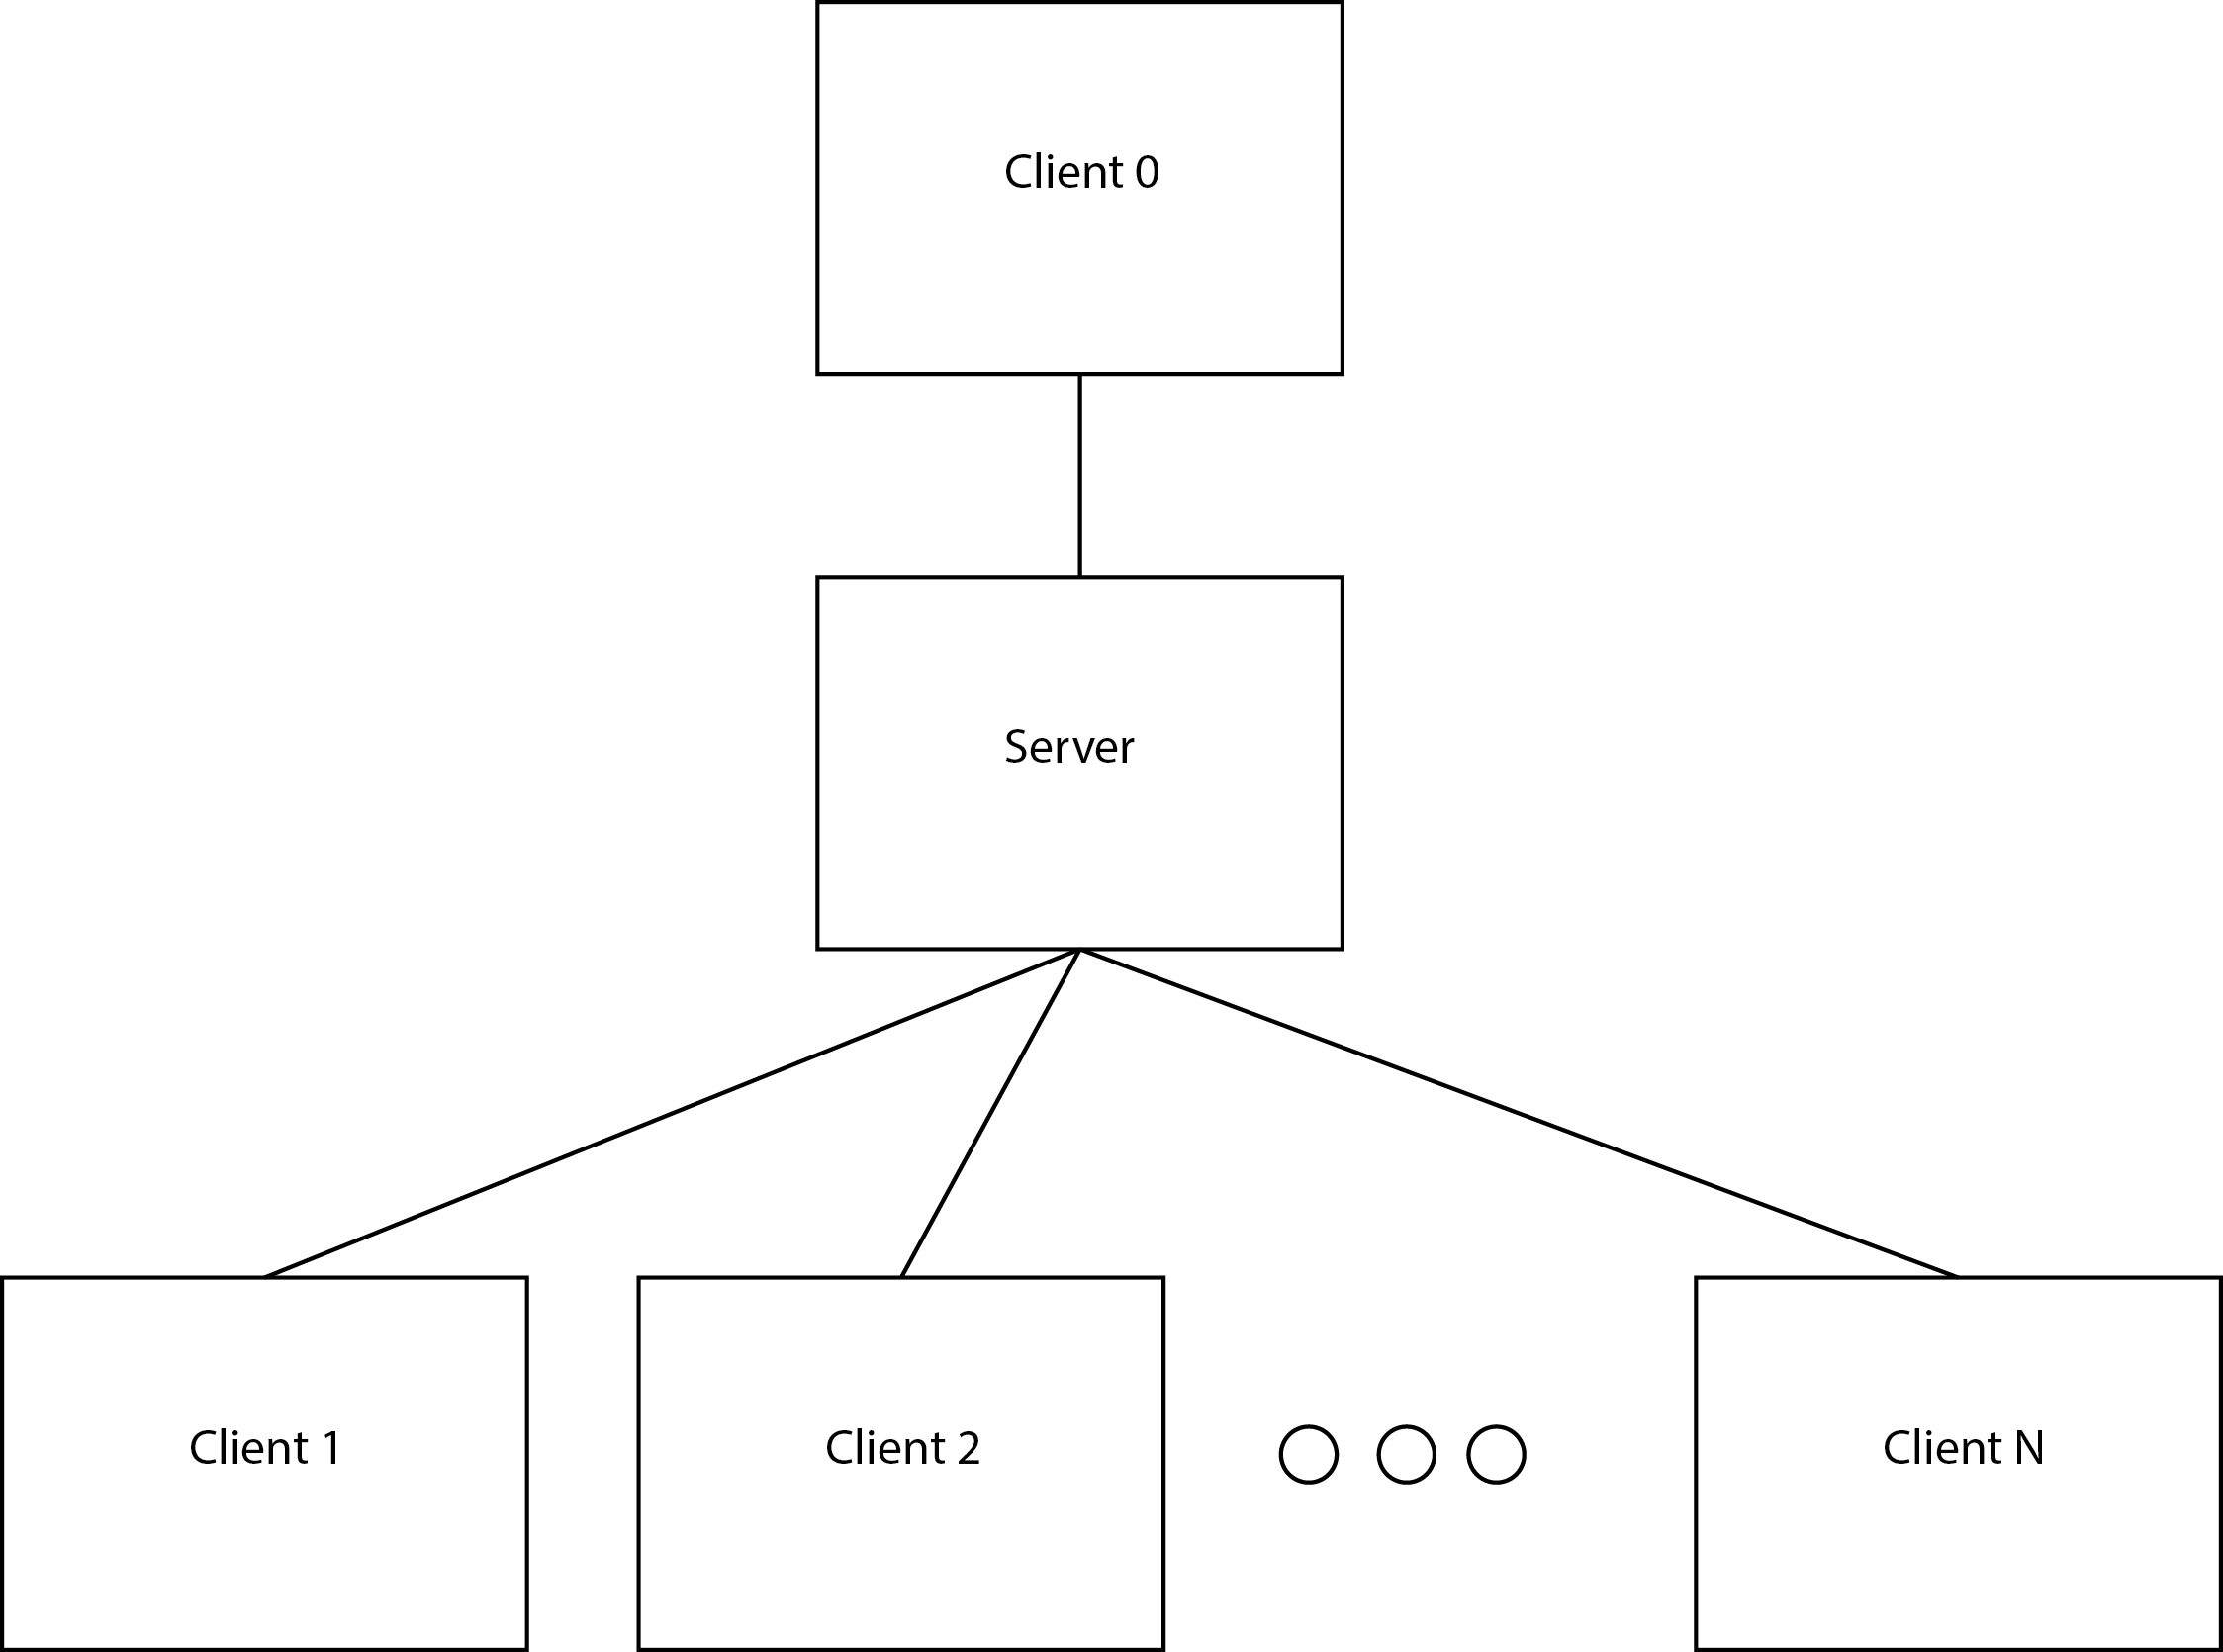
\includegraphics{res/computer_communication_architecture/NetworkTopology.png}
	\caption[Network topology for multiplayer]{Network topology for multiplayer games.}
	\label{fig:serverClientSychNetworkTopology}
\end{marginfigure}

The topology is a typical Star Network, with server in centre, and all clients only connecting to server.
There are $N+1$ player connected, where client 0 is the client that is hosting the server.
Since client 0 is hosting the server, they have special permissions to stop the server at any point, ending the game.
This topology greatly simplifies the requirements of the networking, because every client has to only connect to server, and receive all its updates from 1 single place. 

% protocol for synching game states between client server (command, update)
Figure \ref{fig:loops} gives a good representation how the server and a given client communicate.
This method is \stepTwoName, where both the server and client have a full copy of the model representing the game state.
Their were a variety of benefits from this, the least of which it allowed the clients to scroll around the map without requiring any network traffic.

When the player gives an order, i.e. to move a ship to a given destination, that order is sent to the server in the form of a command.
On the server side, that command is used to 'update' the server's game model. Now the server's game state is at a later version than the clients. The server generates updates that can be applied to all client's game states to bring them to the same version as the server's version.

An example of an update message is: A ship has been given a move order to a location on opposite side of map.
Since their is no simulation on the client side, the ship will only move if the server sends an position update to the clients, moving it slightly closer to its destination. This means that for every time step, every ship that is moving will require an update message send across the network to every client. The move update will look something shown in Table~\ref{table:posupdate}.

\begin{margintable}
    \label{table:posupdate}
    \begin{tabular}{l l l l l}
    \toprule
    \emph{shipID} & \emph{x} & \emph{y} & \emph{direction x} & \emph{direction y} \\ 
    \midrule
    43 & 10 & 15 & 0 & 1 \\
    \bottomrule
    \end{tabular}
    	\vspace{1em}
	\caption[Example of a position update message]{An example of an position update message.}
	\label{tab:positionUpdateExample}
\end{margintable}

Instead of the server telling the client where the ship's destination is, and letting the client move the ship their, the server tells the client when to the next jump location. In the example in Figure \ref{tab:positionUpdateExample} the ship with ID 43 has been given a position update to the new coordinates (10,15), facing North which is (0, 1).

Their are a variety of updates message, depending on which part of the game needs to be updated. 
Originally there was only 3 types of updates:
\begin{description}
\item[addEntity] used for adding an entity to the game. It contains the entity being added to the game.
\item[deleteEntity] used for deleting an entity. An example of use would be when an entity was just blown up. Only contains the entiyID
\item[updateEntity] most common update, used to update an entity. It contains the new entity, and the existing entity is replaced with the entity inside this update.
\end{description}

Having 3 updates provided a very simple design. 
2 out of the 3 updates(addEntity and updateEntity) contains an entity object which is very large in size.
To send an entity object across the network can be very slow and should only be done when necessary.

The addEntity update needs to contain an entity because that entity is currently not in the game, so all the fields of the entity need to be sent across to all the clients. Since addEntity is primarily used at the start of a game when all the entities are loaded into the game, this is not a problem.

However the updateEntity update is sent every time an entity changes location, direction, targets, etc.
Each time an entity's field changes the entire entity must be sent across the network to all the clients.
Not only is this taking up a large amount of bandwidth, but it is sending a large proportion of redundant fields which haven't been changed.
The solution to this was to split the updateEntity update into multiple updates, each one for a common update usage.
The different types of updates to an entity were identifies and a new update message was given to it. 
Table \ref{tab:updateMessageTypes} contains the update messages devised.

\begin{table}
    \begin{tabular}{p{5em} p{15em} p{6em}}
    \toprule
    \emph{Update Type} & \emph{Description} & \emph{Fields} \\
    \midrule
    position & used when both the ship's location and direction has changed & entityID, location, direction \\
    order & when a ship's orders change & entityID, order \\
    goal & when a ship's goal changes & entityID, goal \\
    plan & when a ship's plan to achieve its goal changes & entityID, plan \\
    health & when a ship's hull or shields health changes & entityID, hull health, shield health \\ 
    \bottomrule
    \end{tabular}
    	\vspace{1em}
	\caption[Message update types]{Description of update types.}
	\label{tab:updateMessageTypes}
\end{table}

Now, when a ship's field, say direction changes, the direction update message is used instead of the old entity update message.
This is significantly cheaper with regards to network usage because only the ship's ID and new location are sent.

% network traffic calculation
Their were concerns that the volume of traffic required to maintain all the client's game states updates would still be too great for a playable game.
Therefore a traffic analysis was done to estimate how much network traffic would actually be required.
When assumptions are made concerning the game, such as number of ships, number of game steps per second, etc, worst case scenario will be assumed giving the limitations of the game, IE we will know the maximum number of ships the game can have before the game becomes effects by network bandwidth.



The size of each update message will need to be estimated as well as how frequently that message will be sent.

First, the size of field types will need estimating using language independent types such as int, float, double, etc.
This is done in Table \ref{tab:typeSizes}
\begin{margintable}
    \begin{tabular}{p{5em} p{5em}}
    \toprule
    \emph{Field Type} & \emph{Size (bytes)} \\
    \midrule
    \scalenote{"Int"} & 4 \\ 
    \scalenote{"Float"} & 4 \\
    \scalenote{"Double"} & 8 \\    
    \bottomrule
    \end{tabular}
    	\vspace{1em}
	\caption[field sizes]{Byte sizes of numeric fields.}
	\label{tab:typeSizes}
\end{margintable}

Now we have estimates of size for the different types, we can assign types to each field of the updates messages to estimate the size of each update message, as shown in table \ref{tab:fieldSizes}

\begin{margintable}
    \begin{tabular}{p{5em} p{5em} p{5em}}
    \toprule
    \emph{Field Name} & \emph{Size (bytes)} \\
    \midrule
    entityID & 4 \\ 
    location & 8 \\
    direction & 8 \\ 
    order & 15 \\
    goal & 9 \\ 
    plan & 100 \\ 
    hull & 4  \\ 
    shield & 4  \\  
    \bottomrule
    \end{tabular}
    	\vspace{1em}
    	%todo somebody verify caption please!
	\caption[Size of record types]{Byte sizes of record types.}
	\label{tab:fieldSizes}
\end{margintable}

For the plan field, it was assumed that each action within the plan was approximately 20 bytes, and that the average plan has 5 steps.

Table \ref{tab:updateMessageStats} estimates the size of a message to sent across network.

Now the size and frequency of each update message has been estimated, we calculated how many bytes are sent to a single client every game step.
$$ bytes = 20*1 + 19*0.2 + 14*0.3 + 104*0.3 + 12*0.1 $$
$$ bytes = 60.4 $$

We have $S$ representing the number of game steps per second, and $N$ representing the number of clients connected to server.
The number of bytes the server sends per second is
$$ bytes = S * N * 60.4 $$

We now have a formula to calculate network traffic, we need to apply to to various values of $N$ and $S$, as shown in Table \ref{tab:networkRequirements}.

% s=15, 30, 45, 60, n =2, 4, 8, 16

\begin{margintable}
    \begin{tabular}{p{5em} p{5em} p{5em}}
    \toprule
    \emph{Update Type} & \emph{Size (bytes)} & \emph{Frequency} \\
    \midrule
    position & 20 & 1 \\ 
    order & 19 & 0.2 \\
    goal & 14 & 0.3 \\
    plan & 104 & 0.3 \\
    health & 12 & 0.1 \\   
    \bottomrule
    \end{tabular}
    	\vspace{1em}
	\caption[Update message statistics]{Size of each update message and its average frequency per game step.}
	\label{tab:updateMessageStats}
\end{margintable}

According to these network estimations, when game steps is 60, and there are 16 clients, the network usage per second is 56.62kB/second. This is highly acceptable for running multiplayer over internet as well as LAN networks.

% overview of other strategies
When deciding on how the server and client would synchronise their game states, we had 3 choices:
\begin{itemize}\itemsep-3pt
\item \stepOneName
\item \stepTwoName
\item \stepThreeName
\end{itemize}

\stepTwoName was the method chosen, however it wasn't a clear choice which would be the best since there is no total ordering between them, each one has its own benefits under different circumstances.

% advantages/disadvantages of lockstep
\emph{\stepOneName} is a peer to peer strategy, in which each computer has a full model of the game. Figure \ref{fig:serverClientSychP2P} shows an example of this strategy. 
Their are 4 computers within game. Each client (client 1, client 2, client 3, and client4) have a full copy of the game.
When client 1 updates performs some actions, they must update their game state, and send this update to all other clients.

\begin{margintable}[-8em]
    \begin{tabular}{p{5em} p{5em} p{5em}}
    \toprule
    \emph{Steps Per Second} & \emph{Number of Clients} & \emph{kB/s} \\
    \midrule
    15 & 2 & 1.77 \\
    15 & 4 & 3.54 \\
    15 & 8 & 7.08 \\
    15 & 16 & 14.16 \\
    30 & 2 & 3.54 \\
    30 & 4 & 7.08 \\
    30 & 8 & 14.16 \\
    30 & 16 & 28.31 \\
    45 & 2 & 5.31 \\
    45 & 4 & 10.62 \\
    45 & 8 & 21.23 \\
    45 & 16 & 42.47 \\
    60 & 2 & 7.08 \\
    60 & 4 & 14.16 \\
    60 & 8 & 28.31 \\
    60 & 16 & 56.62 \\
    \bottomrule
    \end{tabular}
    	\vspace{1em}
	\caption[Estimation of network requirements]{
	Estimate of traffic generated for various game setups.}
	\label{tab:networkRequirements}
\end{margintable}

% advantages
%   playable with slow networks
This strategy means players can continue to play games on networks with high latency, without any lag. When packets are delayed, the client can continue to play the game, and the game is updated when the packet arrives.
%   no dedicated server required
No client is picked to act as server, which causes game to end if that selected client disconnects.
Since all clients act as server, any client can disconnect and the game continues, providing more robustness which is highly desirable for games with long game intervals such as Sid Meier's Civilization.
\sidenote{Sid Meier's Civilization is a turn-based strategy game, for more information see civilization.com.}

%todo: Captions here have NOT been checked
\begin{marginfigure}
	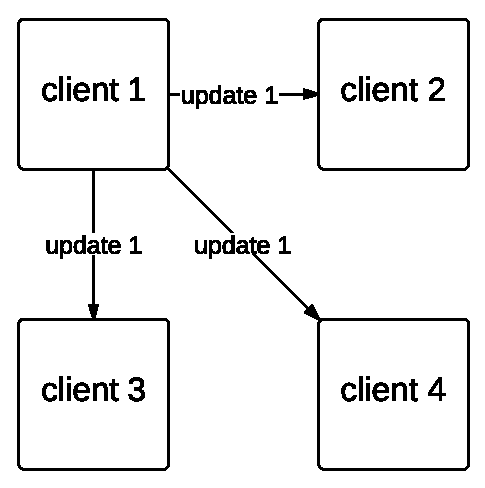
\includegraphics{res/computer_communication_architecture/ServerClientSynchronizationP2P.pdf}
	\caption[\stepOneName : description]{
%	\stepOneName : 4 clients connected. client 1 has just modified its game state, so it send the update to all other clients.
	Lockstep overview. Four clients connect and client 1 modifies its game state, so it send the update to all other clients.
	}
	\label{fig:serverClientSychP2P}
\end{marginfigure}

% \begin{marginfigure}[-30em]
\begin{marginfigure}
	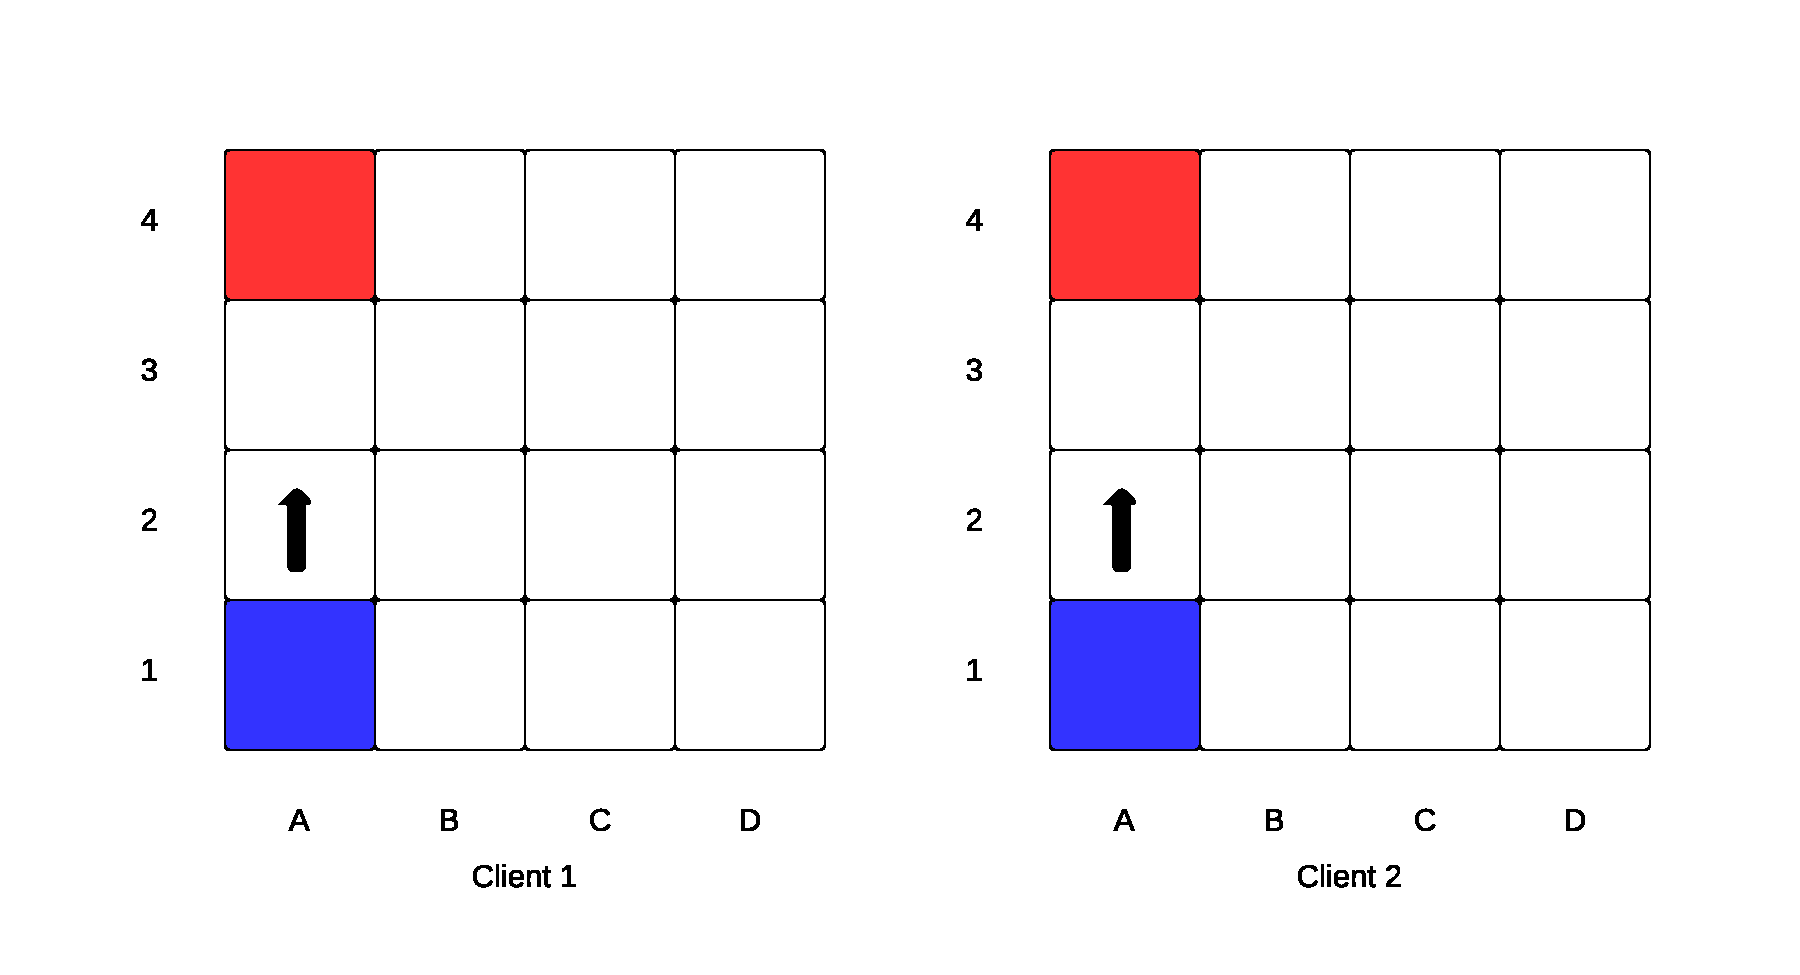
\includegraphics{res/computer_communication_architecture/ServerClientDesynchronisation1.pdf}
	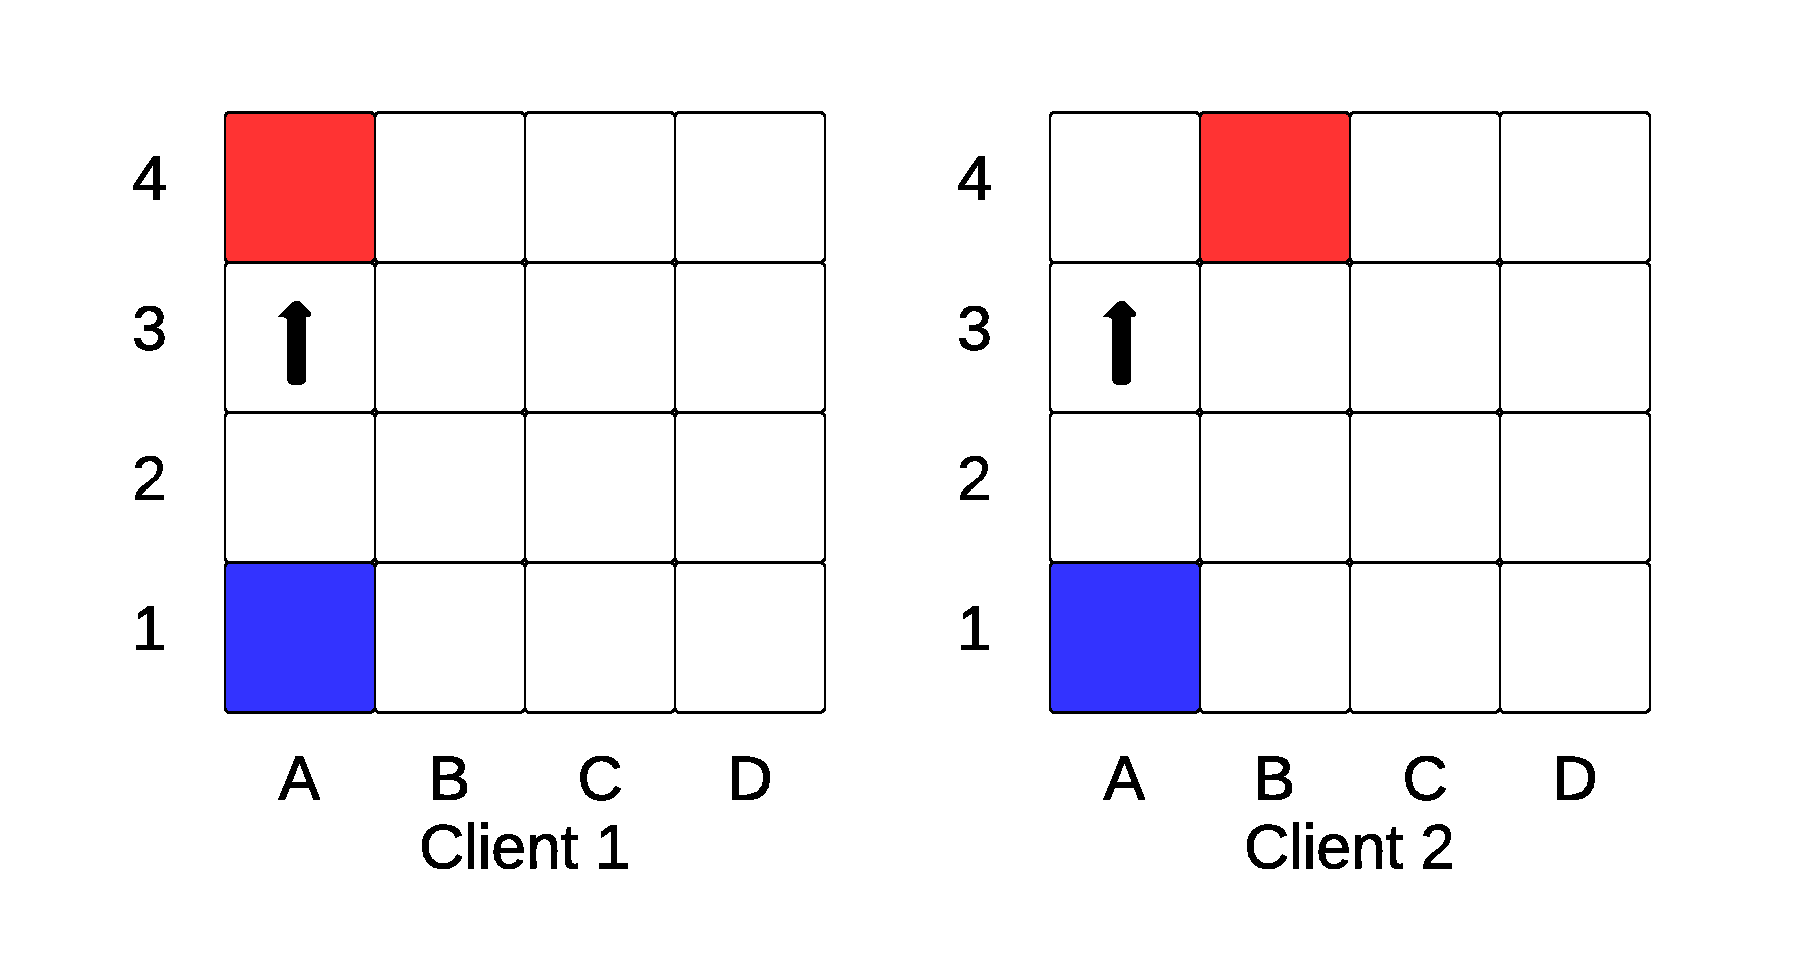
\includegraphics{res/computer_communication_architecture/ServerClientDesynchronisation2.pdf}
	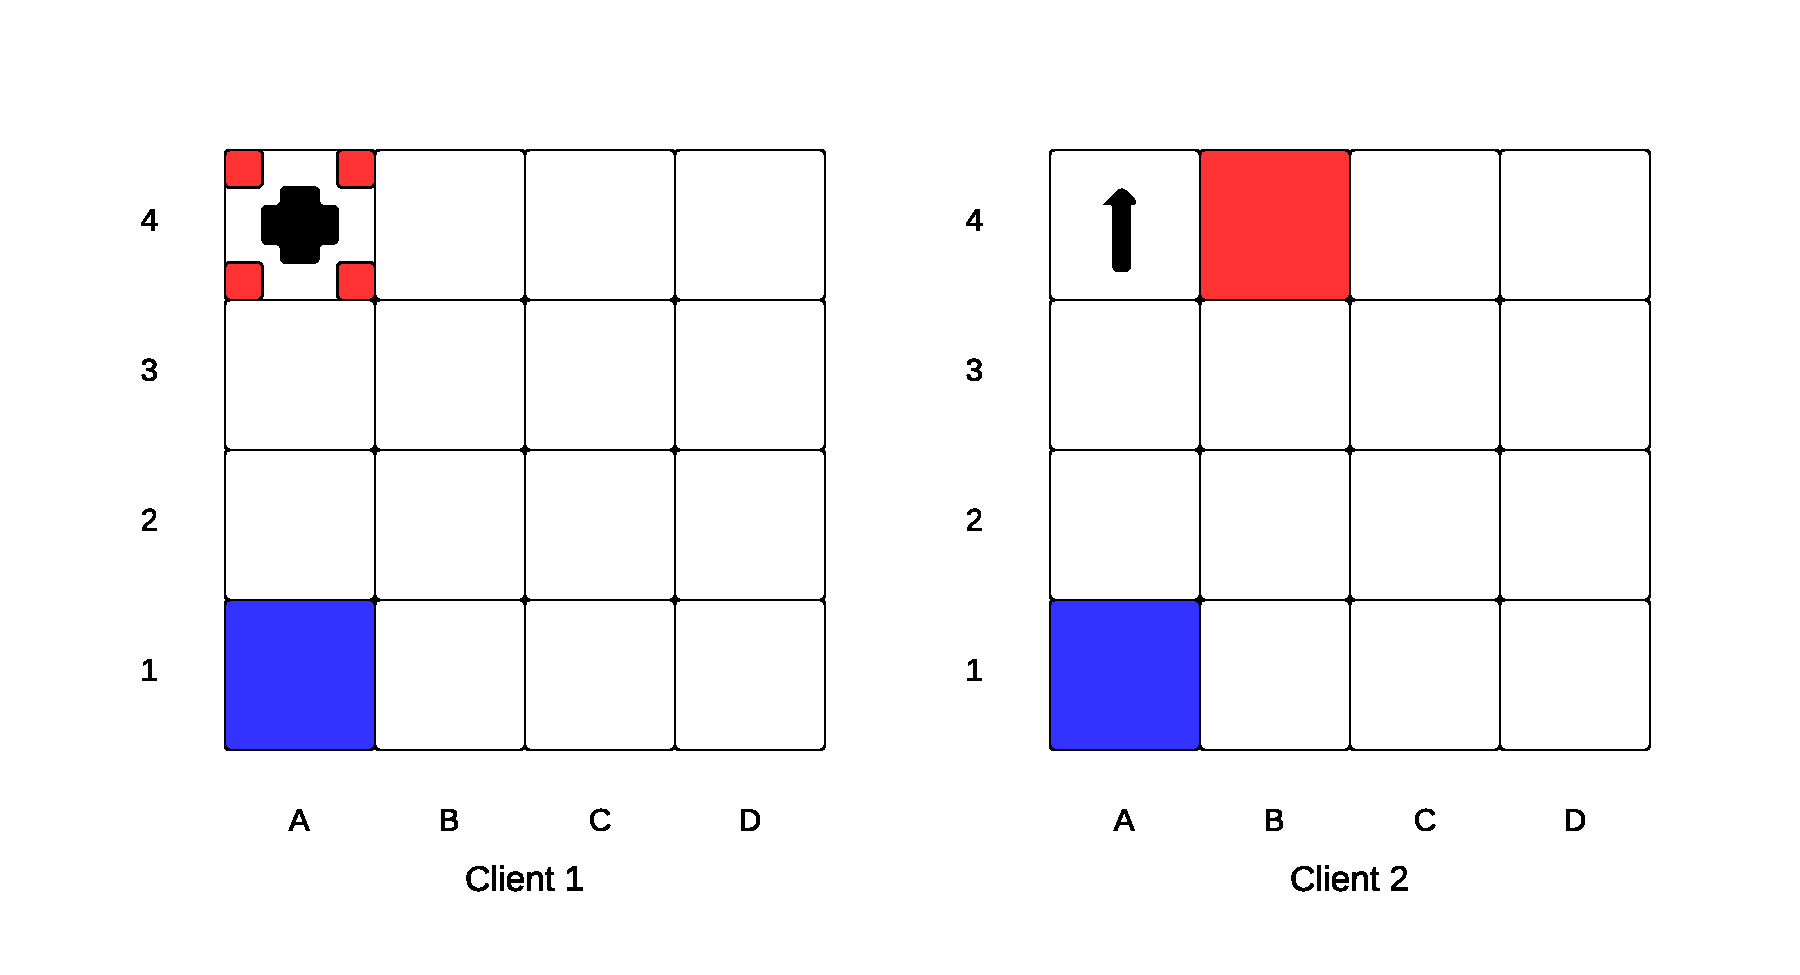
\includegraphics{res/computer_communication_architecture/ServerClientDesynchronisation3.pdf}		
	\caption[\stepOneName : desynchronisation example]{
	\stepOneName : example of desynchronisation when using the \stepOneName strategy. Client 1 on left, client 2 on right. 
	Each diagram represents state of game for that clients at a given time period.	3 diagrams vertically aligned, First one is top, second one is middle, third one is bottom.
	}
	\label{fig:serverClientDesync}
\end{marginfigure}


% disadvantages
%   disynchronization
Maintaining synchronisation when using a peer-2-peer protocol can be very challenging from a technical point of view, with non-determinism being caused by messages being received by clients at different times causing race conditions.
When this happens in a game, it can cause clients game states to desynchronise.
For example, In Figure \ref{fig:serverClientDesync}, there are 2 clients.


% advantages/disadvantages of server client with simulation
\emph{\stepThreeName} is very similar to \stepTwoName with the addition that there is restricted game simulation on the client.
By allowing the clients to simulate their game independent of the server, it greatly reduce the volume of network traffic, because many pieces of information that are sent across can be calculated from the existing game state, such as the ship's next location given its current location and destination.
One of the big issues with \stepTwoName is that the ships move in little 'jumps' where the clients have just received their next position and they move the ship to the next position and the player sees the ship do lots of little jumps before it makes it to its destination. This can be solved with \stepThreeName because the server just needs to send the ship's plan across and the client can then execute the plan.

However it does suffer with problems, because the clients are simulating their game they can fall out of sync with the server, just like \stepOneName. However the architecture means that the clients will never desynchronise too far because the server has the master copy of the game so it will always override the client's version of game state if there ever is a conflict. 
Adding simulation on client side can add much complexity to the client's logic which is one of the primary reasons for choosing the \stepTwoName strategy instead of \stepThreeName.


%
%
%
%----------------------------------- old gay -----------------------------------------
%
%we need to work out how the computers talked to each other very early on
%2 considerations: peer 2 peer, client-server
%  - advantages of peer 2 peer
%  - advantages of peer server-client
%  - why server-client chosen 
%  - issues experienced with server-client
%    - jumpy ship movements
%\end{comment}
%
%The game was designed around being multiplayer, so our first goal was to decide how the player's computers would talk to each other.
%Since their was an arbitrary number of players (greater than 1), We needed a system that would scale, but would also be robust.
%The game was expecting all players to be on the same LAN (Local Area Network), hence a high bandwidth was available for the communications.
%
%There are 3 strategies for the interactions between computers:
%\begin{itemize}
%\item \stepOneName
%\item \stepTwoName
%\item \stepThreeName
%\end{itemize}
%
%
%\begin{marginfigure}
%	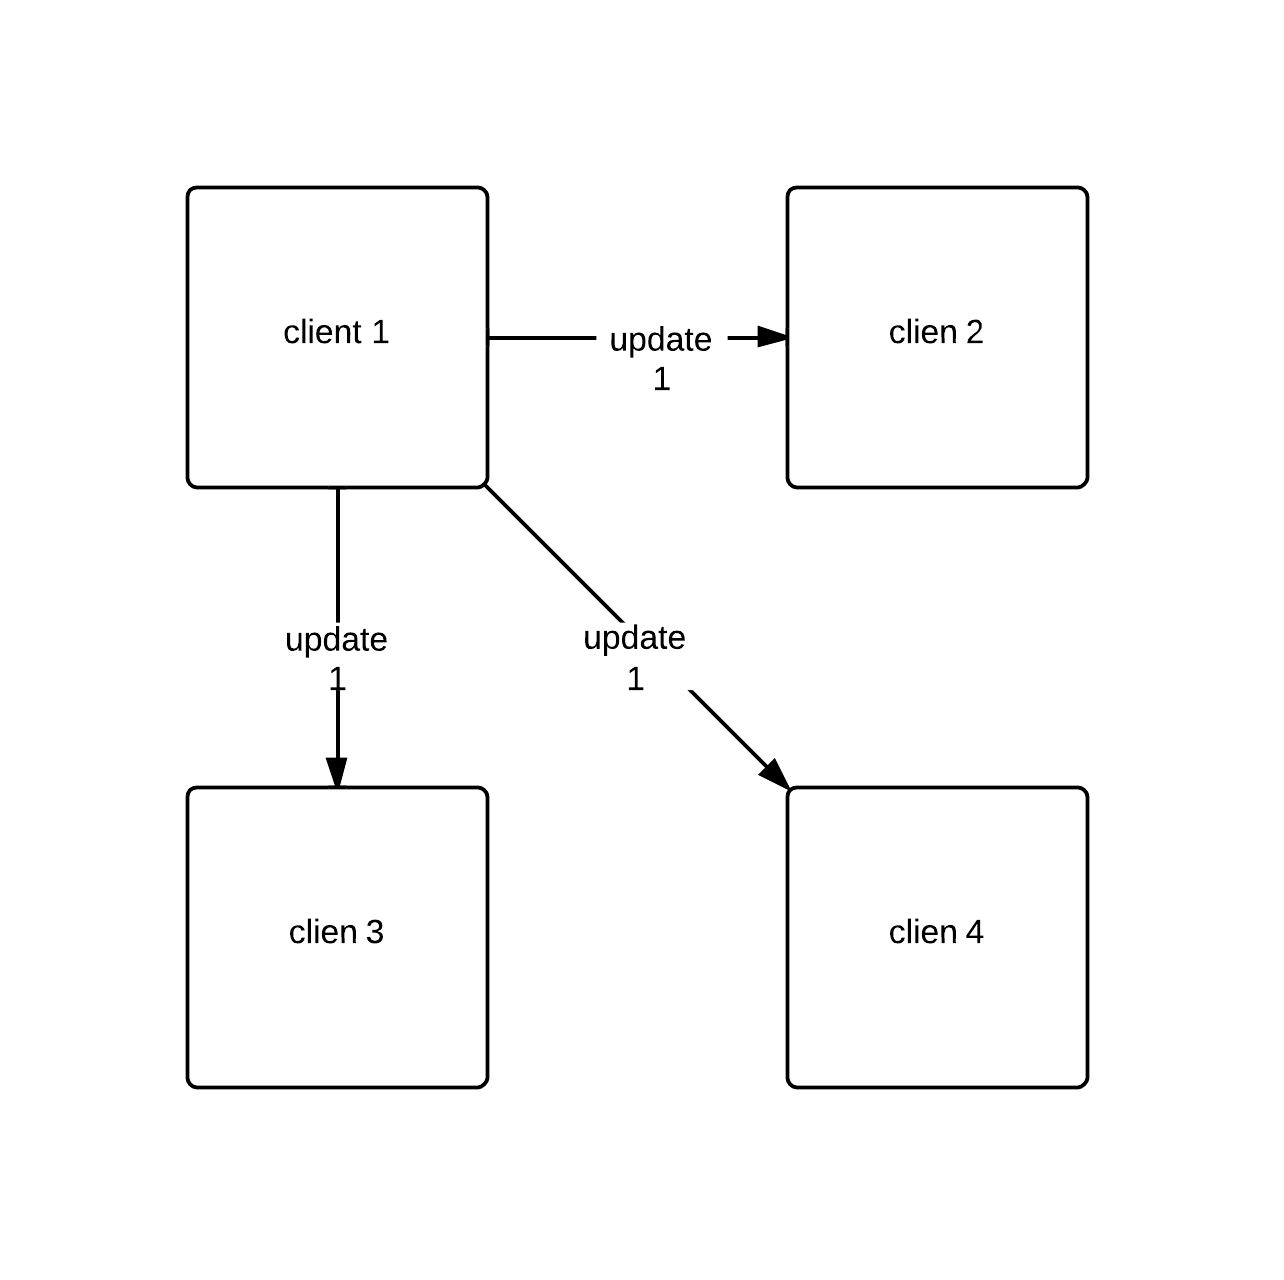
\includegraphics{res/computer_communication_architecture/ServerClientSynchronizationP2P.png}
%	\caption{
%	\stepOneName : 4 clients connected. client 1 has just modified its game state, so it send the update to all other clients.
%	}
%	\label{fig:serverClientSychP2P}
%\end{marginfigure}
%
%% what
%\stepOneName is a peer to peer strategy, in which each computer has a full model of the game. Figure \ref{fig:serverClientSychP2P} shows an example of this strategy. 
%Their are 4 computers within game. Each client (client 1, client 2, client 3, and client4) have a full copy of the game.
%When client 1 updates performs some actions, they must update their game state, and send this update to all other clients.
%
%\begin{marginfigure}[-30em]
%	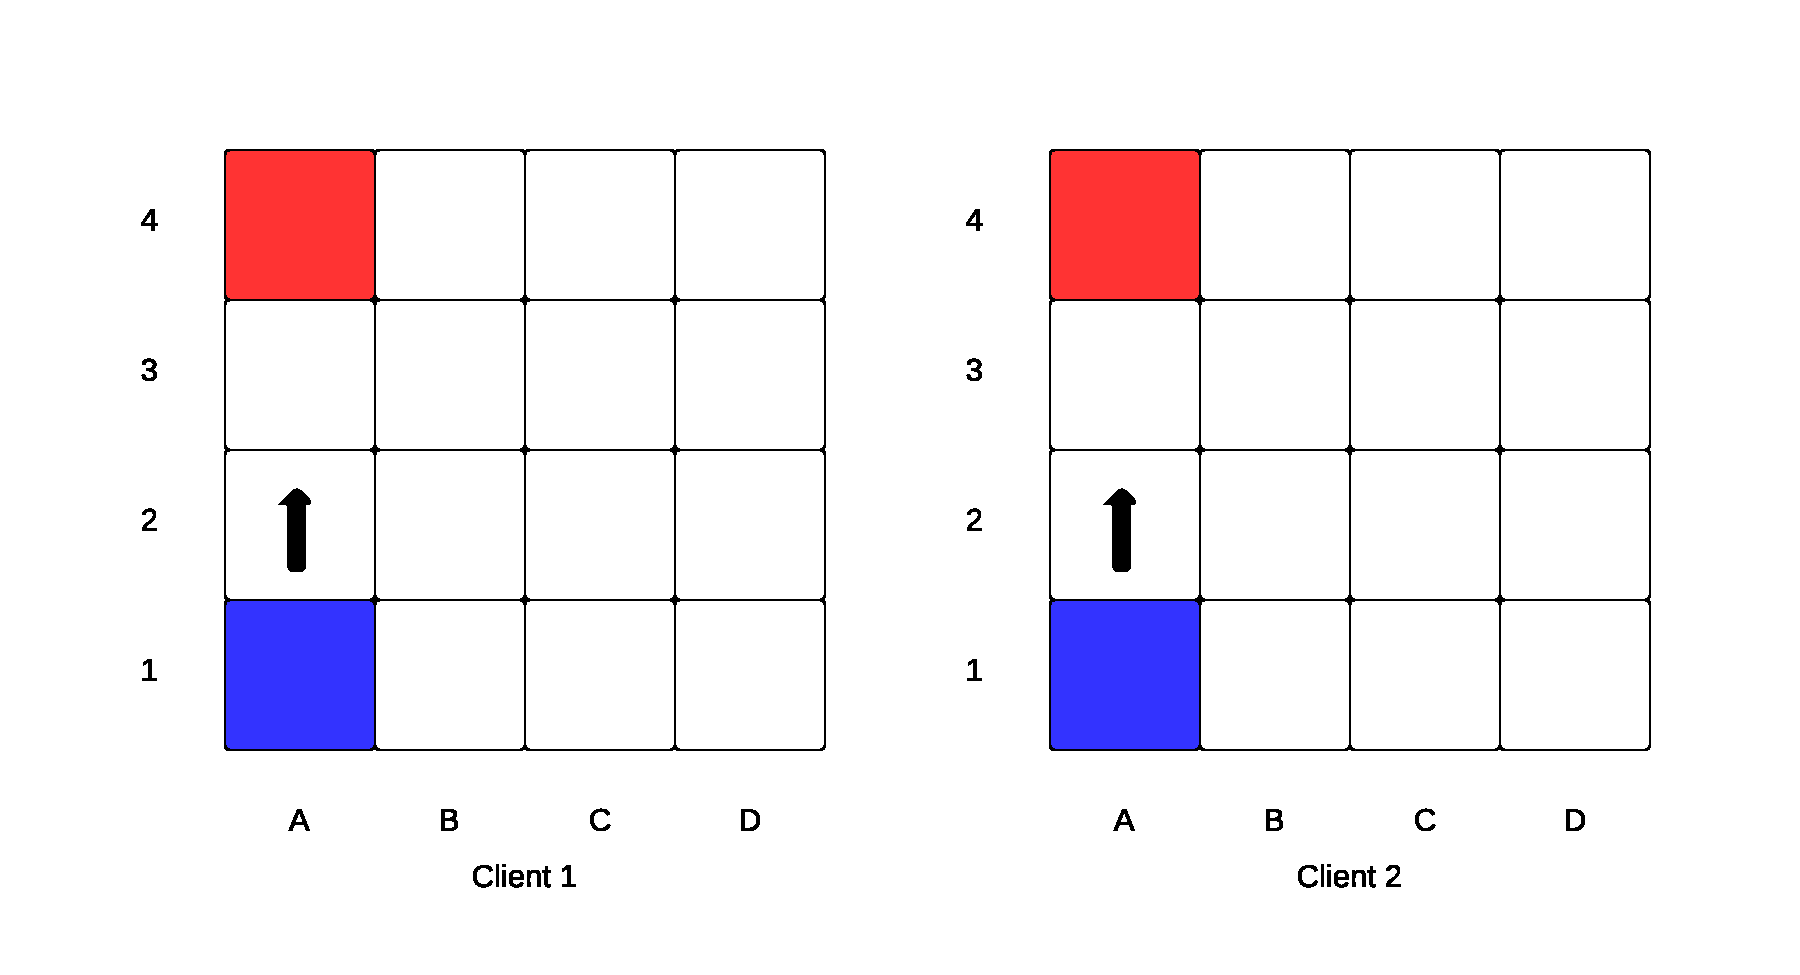
\includegraphics{res/computer_communication_architecture/ServerClientDesynchronisation1.pdf}
%	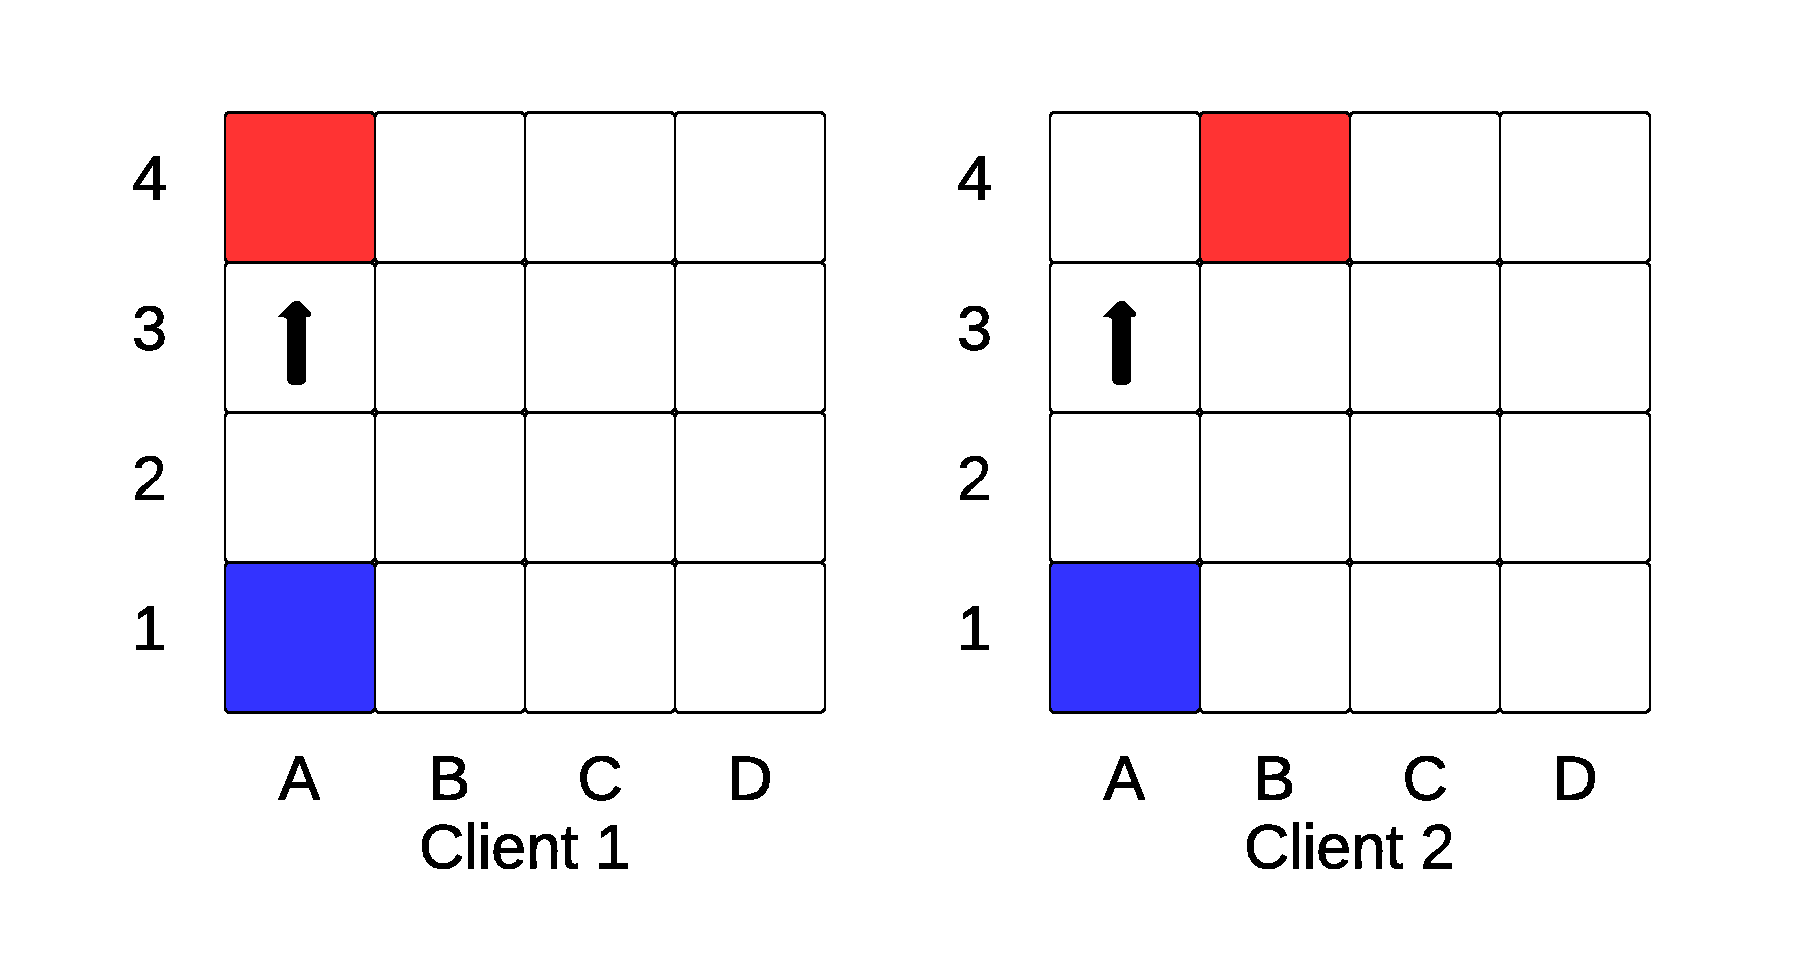
\includegraphics{res/computer_communication_architecture/ServerClientDesynchronisation2.pdf}
%	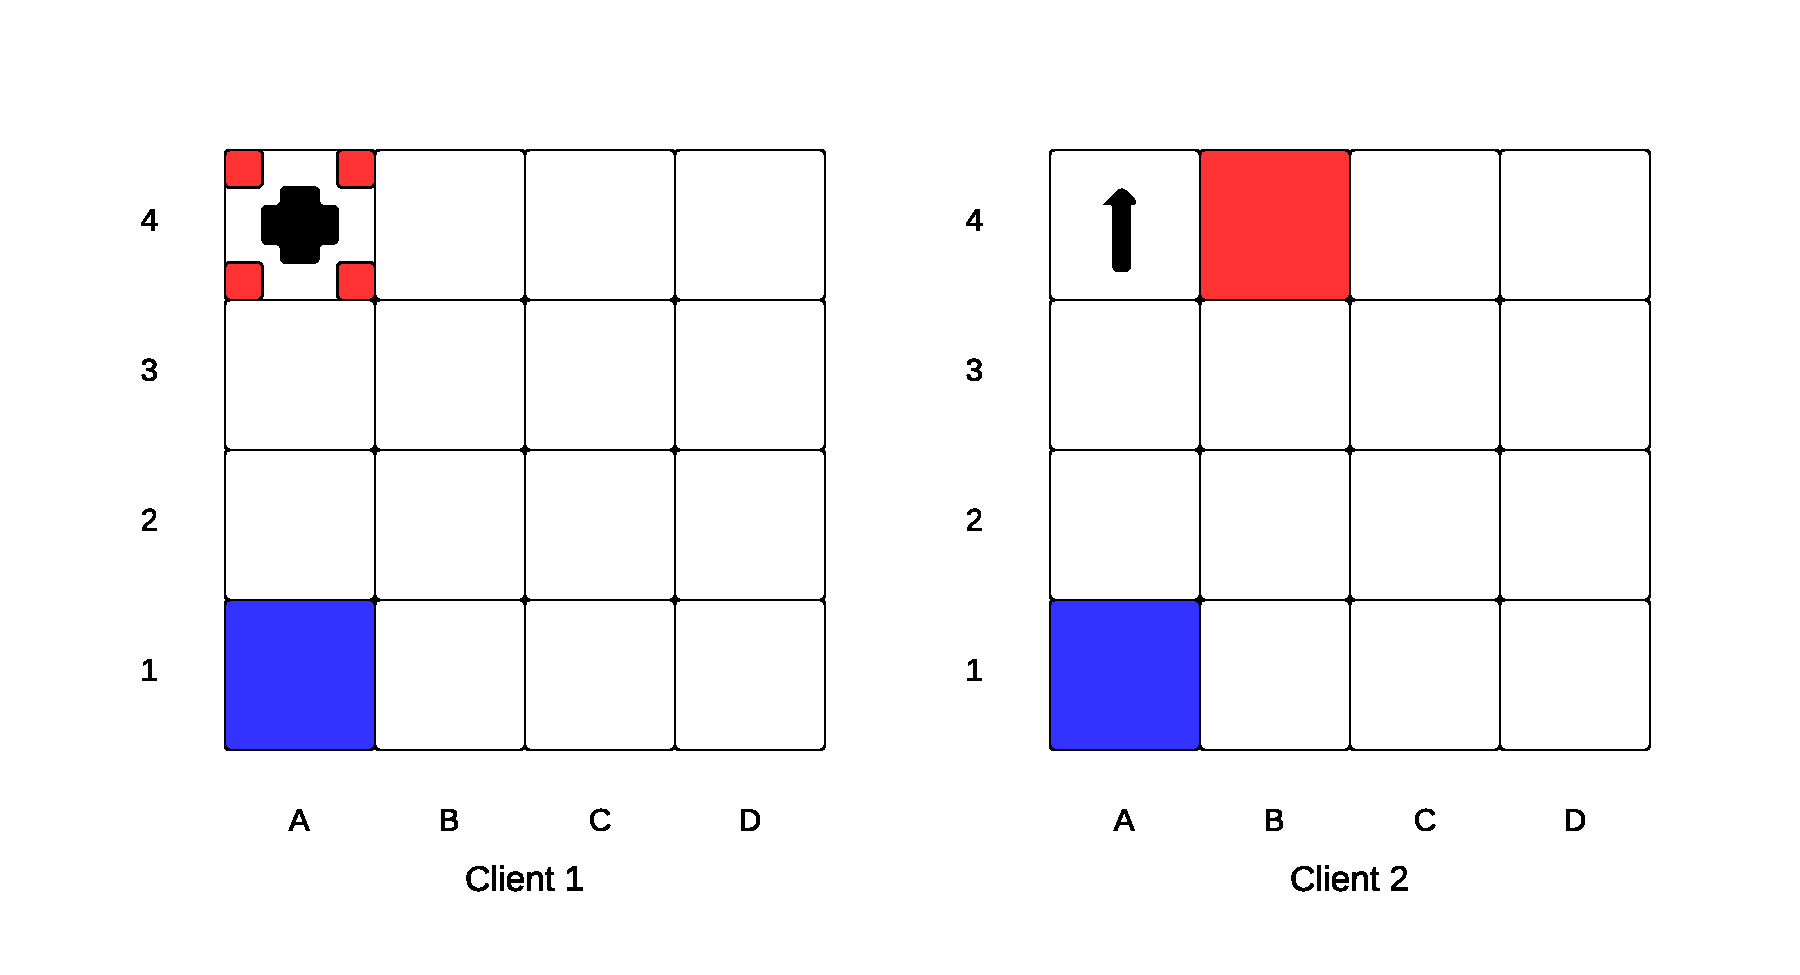
\includegraphics{res/computer_communication_architecture/ServerClientDesynchronisation3.pdf}		
%	\caption{
%	\stepOneName : example of desynchronization when using the \stepOneName strategy. Client 1 on left, client 2 on right. 
%	Each diagram represents state of game for that clients at a given time period.	3 diagrams vertically aligned, First one is top, second one is middle, third one is bottom.
%	}
%	\label{fig:serverClientDesync}
%\end{marginfigure}
%
%% advantages
%%   playable with slow networks
%This strategy means players can continue to play games on networks with high latency, without any lag. When packets are delayed, the client can continue to play the game, and the game is updated when the packet arrives.
%%   no dedicated server required
%No client is picked to act as server, which causes game to end if that selected client disconnects.
%Since all clients act as server, any client can disconnect and the game continues, providing more robustness which is highly desirable for games with long game intervals, such as Civilization series\cite{civilizationInMyPants}.
%
%
%
%% disadvantages
%%   disynchronization
%Maintaining synchronisation when using a peer-2-peer protocol can be very challenging from a technical point of view, with non-determinism being caused by messages being received by clients at different times causing race conditions.
%When this happens in a game, it can cause clients game states to desynchronise.
%For example, In Figure \ref{fig:serverClientDesync}, there are 2 clients.
%%   corrupted client can effect the entire game
%
%
%
%% res/computer_communication_architecture
%
%
%
%
%% lockstep
%%   - each client has the master copy of the world
%%   - when a client does something, it tells all others
%%   - problems:
%%     - desycnhronization
%%     - currupted client fucks up everyone
%
%% simple server client
%%   - it's what we've implemented
%%   - no simulation on clients
%%   - 1 server that has master copy
%%   - server does all processing and sends updates to clients
%%   - clients just render the world and send commands to server
%
%% server client with simulation
%%   - similar to simple server client but client does 'some' simulation. They in no way can effect the world.
%%   - for instance if client knows ships destination and current location it can render the ship graciously moving instead of jumping on every update.
%

\end{comment}
